
\documentclass[fleqn,addpoints]{exam}

\usepackage{units} 
\usepackage{graphicx}
\usepackage[fleqn]{amsmath}
\usepackage{cancel}
\usepackage{float}
\usepackage{mdwlist}
\usepackage{booktabs}
\usepackage{cancel}
\usepackage{polynom}
\usepackage{caption}
\usepackage{fullpage}
\usepackage{xfrac}
\usepackage{enumerate}

\everymath{\displaystyle}

\printanswers

\ifprintanswers
  \usepackage{2in1, lscape}
\fi

\title{Math 141 Chapter Three Exam}
\date{May 29, 2013}
\author{}

\begin{document}

  \maketitle  

  % \ifprintanswers
  %   \else
  %   \vspace{0.2in}
  %   \makebox[\textwidth]{Name:\enspace\hrulefill}
  %   \vspace{0.2in}

  %   \begin{center}
  %   \gradetable[h][pages]
  %   \bonusgradetable[h][pages]
  %   \end{center}
  % \fi

  % \vspace{1 cm}

  % \ifprintanswers
  % \else
  %   \pagebreak
  % \fi

  \begin{questions}
    \uplevel{\section{Questions}}
    %% \uplevel{ \section{Polynomial Long Division} }

    \question Evaluate each expression and write the result in the form $a + bi$
      \begin{parts}
          \part[5]
          \[
            \frac{\sqrt{-4}}{\sqrt{-9} \sqrt{-2}}
          \]

          \begin{solution}
            \begin{align*}
              \frac{\sqrt{-4}}{\sqrt{-9} \sqrt{-2}} &= \frac{2i}{3i \cdot i \sqrt{2}} \\
                                                    &= \frac{2i}{-3 \sqrt{2}} \\
                                                    &= \boxed{- \frac{\sqrt{2}}{3} i} \\
            \end{align*}
          \end{solution}

        \ifprintanswers
          \pagebreak
        \fi

        \part[5]
          \[
            \frac{5 + i}{4 - 2i}
          \]

          \begin{solution}
            \begin{align*}
              \frac{5 + i}{4 - 2i} &= \frac{5 + i}{4 - 2i} \left( \frac{4 + 2i}{4 + 2i} \right) \\
                                   &= \frac{20 + 14i + 2i^2}{16 - 4i^2} \\
                                   &= \frac{18 + 14i}{20} \\
                                   &= \boxed{\frac{9}{10} + \frac{7}{10} i} \\
            \end{align*}
          \end{solution}

      \end{parts}

    \question Use either synthetic or polynomial long division to find the quotient and remainder and write the result
      in the form: $Q(x) + \frac{R(x)}{D(x)}$.

      \begin{parts}
        
        \part[5]
          \[
            \frac{3x^3 - 4x + 7}{x + 2}
          \]

        \begin{solution}
          \[
            \polyhornerscheme[x = -2]{3x^3 - 4x + 7}
          \]

          \[
            \boxed{3x^2 - 6x + 8 - \frac{9}{x + 2} }
          \]
        \end{solution}

        \part[5]
          \[
            \frac{6x^4 - 6x^3 + 5x^2 - 3x + 8}{2x^2 + 1}
          \]

          \begin{solution}
            \[
              \polylongdiv{6x^4 - 6x^3 + 5x^2 - 3x + 8}{2x^2 + 1}
            \]

            \[
              \boxed{3x^2 - 3x + 1 + \frac{7}{2x + 1}}
            \]

          \end{solution}
      \end{parts}

    \question[10] Find all rational zeros of $f$.
    \[
      f(x) = 2x^3 - 14x - 12
    \]

    \begin{solution}
      It's a little easier to find the zeros if you factor out a 2:
      \[
        f(x) = 2x^3 - 14x - 12 = 2\left( x^3 - 7x - 6 \right)
      \]

      From the Rational Zeros Theorem, the candidates are: 
      \[
        x = \{\pm 1, \pm 2, \pm 3, \pm 6 \}
      \]

      \begin{align*}
        x^3 - 7x - 6 &= (x + 1) (x^2 - x + 6) \\
                     &= (x + 1) (x - 3) (x + 2) \\
      \end{align*}

      \[
        \boxed{x = \{-1, -2, 3 \}}
      \]

    \end{solution}

    \question[10] Find all rational zeros of $f$.
    \[
      f(x) = 2x^3 - 7x^2 - 17x + 10
    \]

    \begin{solution}
      From the Rational Zeros Theorem, the candidates are: 
      \[
        x = \{\pm 1, \pm 2, \pm 5, \pm 10, \pm \frac{1}{2}, \pm \frac{5}{2}  \}
      \]

      \begin{align*}
        2x^3 - 7x^2 - 17x + 10 &= (x + 2) (2x^2 - 11x + 5) \\
                               &= (2x - 1) (x + 2) (x - 5) \\
      \end{align*}
      \[
        \boxed{x = \{-2, \frac{1}{2}, 5 \}}
      \]
    \end{solution}

    \ifprintanswers
      \pagebreak
    \fi

    \question[10] Factor $f$ completely.
    \[
      f(x) = x^3 - 5x^2 + 11x - 15
    \]

    \begin{solution}
      From the Rational Zeros Theorem, the candidates are: 
      \[
        x = \{\pm 1, \pm 3, \pm 5, \pm 15 \}
      \]

      The only rational solution is 3:
      \[
        x^3 - 5x^2 + 11x - 15 = (x - 3) (x^2 - 2x + 5) 
      \]

      Use the quadratic formula to find the remaining solutions:
      \begin{align*}
        x &= \frac{2 \pm \sqrt{4 - 4 \cdot 5}}{2} \\
          &= \frac{2 \pm \sqrt{-16}}{2} \\
          &= \frac{2 \pm 4i}{2} \\
          &= 1 \pm 2i \\
      \end{align*}
      
      The solutions are:
      \[
        x = \{ 3, 1 + 2i, 1 - 2i \}
      \]

      So the complete factorization is:
      \begin{align*}
        f(x) &= (x - 3)(x - (1 + 2i))(x - (1 - 2i)) \\
             &= \boxed{(x - 3)(x - 1 - 2i)(x - 1 + 2i)} \\
      \end{align*}

    \end{solution}

    \ifprintanswers
      \pagebreak
    \fi

    \question[5] Use the Remainder Theorem to evaluate $f(2)$.
      \[
        f(x) = x^5 + 4x^4 - 15x^3 + 12x - 3
      \]

      \begin{solution}
        \[
          \polyhornerscheme[x = 2]{x^5 + 4x^4 - 15x^3 + 12x - 3}
        \]

        $\boxed{f(2) = -3}$

      \end{solution}

    \question[5] Use Decartes' Rule of Signs to determine the possible number of positive and negative real zeros.
      \[
        f(x) = 2x^5 + 3x^3 - x^2 - x + 7
      \]

      \begin{solution}
        There are 2 changes of sign in $f(x)$ so there are \fbox{2 or 0 positive real zeros}.

        \[
          f(-x) = -2x^5 - 3x^3 - x^2 + x + 7
        \]
        $f(-x)$ only has one change of sign so there is \fbox{1 negative real zero.}

      \end{solution}

    \ifprintanswers
      \pagebreak
    \fi

    \question[7] Find a polynomial of degree 3 with integer coefficients and zeros $3i$ and $2$.
    \begin{solution}
      \begin{align*}
        f(x) &= (x - 3i)(x + 3i)(x - 2) \\
             &= (x^2 + 9)(x - 2) \\
             &= \boxed{x^3 - 2x^2 + 9x - 18} \\
      \end{align*}
    \end{solution}

    \question $f(x) = x^3 + 3x^2 - 4x - 12$
      \label{graph1}

      \begin{parts}
        \part[3] Find the x-intercepts.
          \begin{solution}
            \begin{align*}
              x^3 + 3x^2 - 4x - 12         &= 0 \\
              x^2( x + 3) - 4(x + 3)       &= 0 \\
              \left(x^2 - 4 \right)(x + 3) &= 0 \\
              (x + 2)(x - 2)(x + 3)        &= 0 \\
              \\
              x &= \{ -3, -2, 2 \} \\
            \end{align*}
            The x-intercepts are: \fbox{$(-3, 0)$, $(-2, 0), (2, 0)$}
          \end{solution}
        \part[2] Find the y-intercept.
        \begin{solution}  
          $f(0) = -12$ so the y-intercept is \fbox{(0, -12)}.
        \end{solution}

        \part[3]
          Graph $f$.

          \ifprintanswers
            \begin{figure}[H]
              \centering
                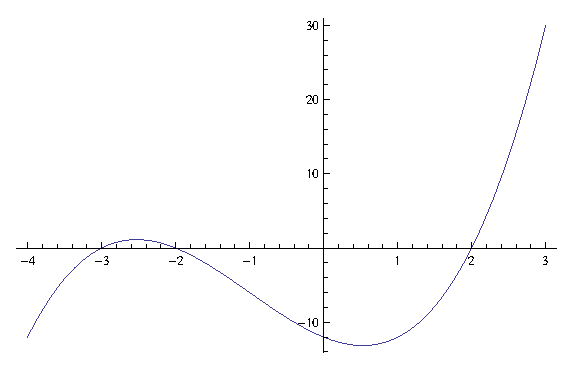
\includegraphics[scale=0.8]{graph1.eps}
              \caption*{Question \ref{graph1}}
            \end{figure}
          \fi

      \end{parts}

    \question
      \label{graph2}

      \[
        f(x) = \frac{2x^2 - 2x - 4}{x^2 + 2x - 3}
      \]

      \begin{parts}
        \part[2] Find the x-intercepts.
          \begin{solution}
            \begin{align*}
              2x^2 - 2x - 4  &= 0 \\
              x^2 - x - 2    &= 0 \\
              (x - 2)(x + 1) &= 0 \\
              \\
              x &= \{ -1, 2 \} \\
            \end{align*}
            The x-intercepts are: \fbox{$(-1, 0)$ and $(2, 0)$}
          \end{solution}

        \part[2] Find the y-intercept.
        \begin{solution}
          $f(0) = \frac{4}{3}$

          The y-intercept is \fbox{$\left( 0, \frac{4}{3} \right)$}

        \end{solution}

        \part[2] Find the vertical asymptote(s).
          \begin{solution}
            \begin{align*}
              x^2 + 2x - 3   &= 0 \\
              (x - 1)(x + 3) &= 0 \\
              \\
              x &= \{ -3, 1 \} \\
            \end{align*}

            The vertical asymptotes are \fbox{$x = -3$ and $x = 1$}.

          \end{solution}

        \part[2] Find the horizontal or slant asymptote(s).
        \begin{solution}
          Since the degree of the numerator is equal to the degree of the denominator, there is a horizontal asymptote
          at \fbox{$y = 2$}
        \end{solution}

        \part[4]
          Graph $f$.

          \ifprintanswers
            \begin{figure}[H]
              \centering
                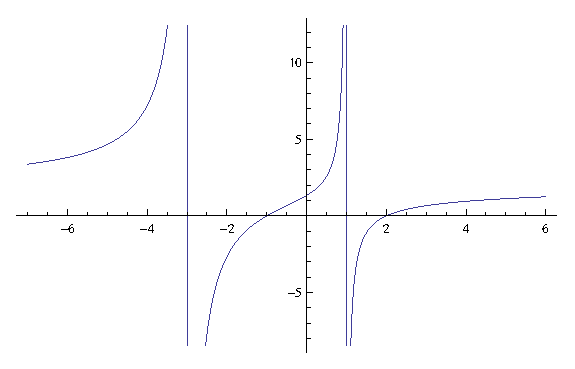
\includegraphics[scale=1.0]{graph2.eps}
              \caption*{Question \ref{graph2}}
            \end{figure}
          \fi

      \end{parts}

    \question
      \label{graph3}

      \[
        f(x) = \frac{x^2 + 2x + 2}{x + 1}
      \]

      \begin{parts}
        \part[2] Find the x-intercepts.
          \begin{solution}
            $x^2 + 2x + 2$ has no real solutions so there aren't any x-intercepts
          \end{solution}

        \part[2] Find the y-intercept.
        \begin{solution}

          $f(0) = 2$ so the y-intercept is \fbox{$(0, 2)$}.

        \end{solution}

        \part[2] Find the vertical asymptote(s).
          \begin{solution}
            \fbox{$x = -1$}
          \end{solution}

        \part[3] Find the horizontal or slant asymptote(s).
        \begin{solution}
          Since the degree of the numerator is exactly one more than the degree of the denominator, there is a slant asymptote.

          \[
            \polyhornerscheme[x = -1]{x^2 + 2x + 2}
          \]

          The slant asymptote is: \fbox{$y = x + 1$}

        \end{solution}

        \ifprintanswers
          \pagebreak
        \fi

        \part[4]
          Graph $f$.

          \ifprintanswers
            \begin{figure}[H]
              \centering
                
\includegraphics[scale=0.9]{graph3.eps}
              \caption*{Question \ref{graph3}}
            \end{figure}
          \fi

      \end{parts}

      \uplevel{\section{Extra Credit}}

      \bonusquestion[10]
        Multiply three consecutive integers together and then add the second integer to the product.  Use synthetic
        division to help prove that the sum is the cube of an integer and determine which integer.

        \begin{solution}
          If $x$ is the first number, the other two numbers are $x + 1$ and $x + 2$.  When you multiply the three
          numbers and add the second one, you get:
          \[
            x(x + 1)(x + 2) + (x + 1) = x^3 + 3x^2 + 3x + 1
          \]

          The only possible zeros are $x = \pm 1$.  If you try both of them, you find that $(x + 1)$ is the only
          factor and:
          \[
            x^3 + 3x^2 + 3x + 1 = (x + 1)^3
          \]

          Another way of seeing the same thing without doing any division is to factor $(x+1)$ out of the original
          equation and simplify:
          \begin{align*}
            x(x + 1)(x + 2) + (x + 1) &= (x+1) [ x(x+2) + 1 ] \\
                                      &= (x + 1) \left( x^2 + 2x + 1 \right) \\
                                      &= (x + 1) (x + 1)^2 \\
                                      &= (x + 1)^3 \\
          \end{align*}
          
        \end{solution}
  \end{questions}

\end{document}

